\begin{columns}
\begin{column}{.65\textwidth}
Vi diskretiserer henholdsvis integralene
\[
\int_S \phi \partial_{\nhat} \ln{r} \,\dee S \approx \sum_{m = 1}^{N} \phi_m \int_{S_m} \partial_{\nhat} \ln{r} \,\dee S;
\]
\[
\int_{S} \ln{r} \partial_{\nhat} \phi \,\dee S \approx \sum_{m = 1}^{N} \partial_{\nhat} \phi_m \int_{S_m} \ln{r} \,\dee S.
\]
\end{column}
\begin{column}{.35\textwidth}
  \begin{figure}[H]
\scalebox{.65}{%
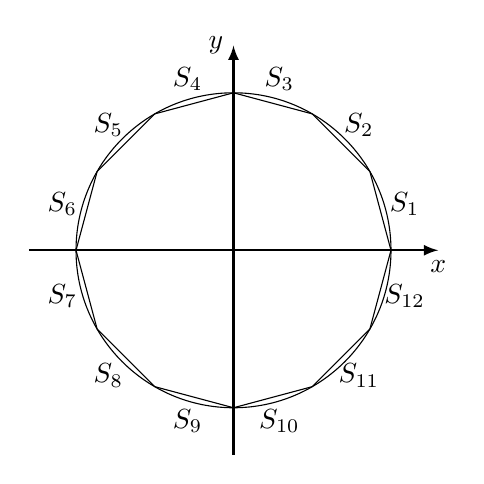
\begin{tikzpicture}
    \begin{scope}[scale = 2]
        \draw[thick, -latex] (-1.3,0)--(1.3,0) node[below]{$x$};
        \draw[thick, -latex] (0,-1.3)--(0,1.3) node[left]{$y$};
        \draw (0,0) circle (1);
        \def\angel{30}
        \foreach \x in {1,...,12}
        {
            \draw ({cos((\x-1)*\angel)}, {sin((\x-1)*\angel)})--({cos(\x*\angel)}, {sin(\x*\angel)});
            \node at ({1.125*cos((2*\x-1)*\angel/2)}, {1.125*sin((2*\x-1)*\angel/2)}) {$S_{\x}$};
        }
    \end{scope}
\end{tikzpicture}}
\end{figure}
\end{column}
\end{columns}
